% Ubah judul dan label berikut sesuai dengan yang diinginkan.
\section{Methodology}
\label{sec:arsitektur}

\subsection{You Only Look Once (YOLO) Model}
\label{subsec:yolo_base}

\par You Only Look Once or YOLO is a very fast multi-object detection algorithm that was introduced by Redmond et al in 2015 through their book You Only Look Once: Unified, Real-Time Object Detection \cite{redmon2016you}. The Convolutional Neural Network (CNN) is the basis of this YOLO detection system. YOLO performs object detection by considering it as a single regression problem that is taken directly from the pixels in the image into a bounding box marker of coordinates and probability of classification. That way it only needs to be checked once on the image to detect or identify. \cite{redmon2016you} YOLO combines several components of the object text into a single neural network that uses features from all parts of the image to predict each bounding box while simultaneously predicting all bounding boxes in all types of classifications. The design of YOLO allows for end-to-end training and real-time detection speed.

\par The YOLO system itself divides the input image into an S x S grid. The role of the grid here is for later, that is, if a certain grid becomes the center of the object, then that grid will be useful for detecting the object earlier.

\par Each grid predicts each bound box and the value of the possible classification or confidence score of the bounding box. This value represents how "sure" the model is of the object detected in the bounding box and how accurate its prediction is.

\par There are five predicted values in each bounding box, namely: x, y, w, h, and confidence. X and Y represent the center of the bounding box. W and H represent the relative predicted Weight and Height of the entire image. Then the confidence score itself represents the IOU between the predicted box and the ground truth box \cite{redmon2016you}.

\subsubsection{YOLOv5}
\label{subsecsec:yolov5}

\par YOLOv5 is an updated version of YOLO which was created in 2020 by Glenn Jocher \cite{glenn_jocher_yolov5}. Based on the Github repository for YOLOv5 by Glenn Jocher, the network structure of YOLOv5 is divided into 3 main parts, namely Backbone, Neck, and Head modules. As can be seen in Figure \ref{fig:yolov5network}. 

\par The network structure of YOLOv5 starts from the Backbone module where the input image is passed first to extract features from the image whose structure is based on CSP-Darknet53. But before going through the Backbone, the input image are being pass through the Focus structure. Inside the backbone, the input go through several  Bottleneck CSP Networks (Cross Stage Partial Networks) and then  and Spatial Pyramid Pooling (SPP). The main purpose of the Spatial Pyramid Pooling block is to generate output with the same size regardless of the size of the input frame. The result of feature extraction from Backbone is then used to generate \emph{feature pyramid} in the Neck module which is a structure based on PANet (Path Aggregation Network). Finally, in the Head Module, the information needed to draw bounding box and to tell what class is being detected is generated here which includes some information, namely: class, coordinates, and confidence score.

\begin{figure*} [ht]
  \centering
  % Ubah sesuai dengan nama file gambar dan ukuran yang akan digunakan.
  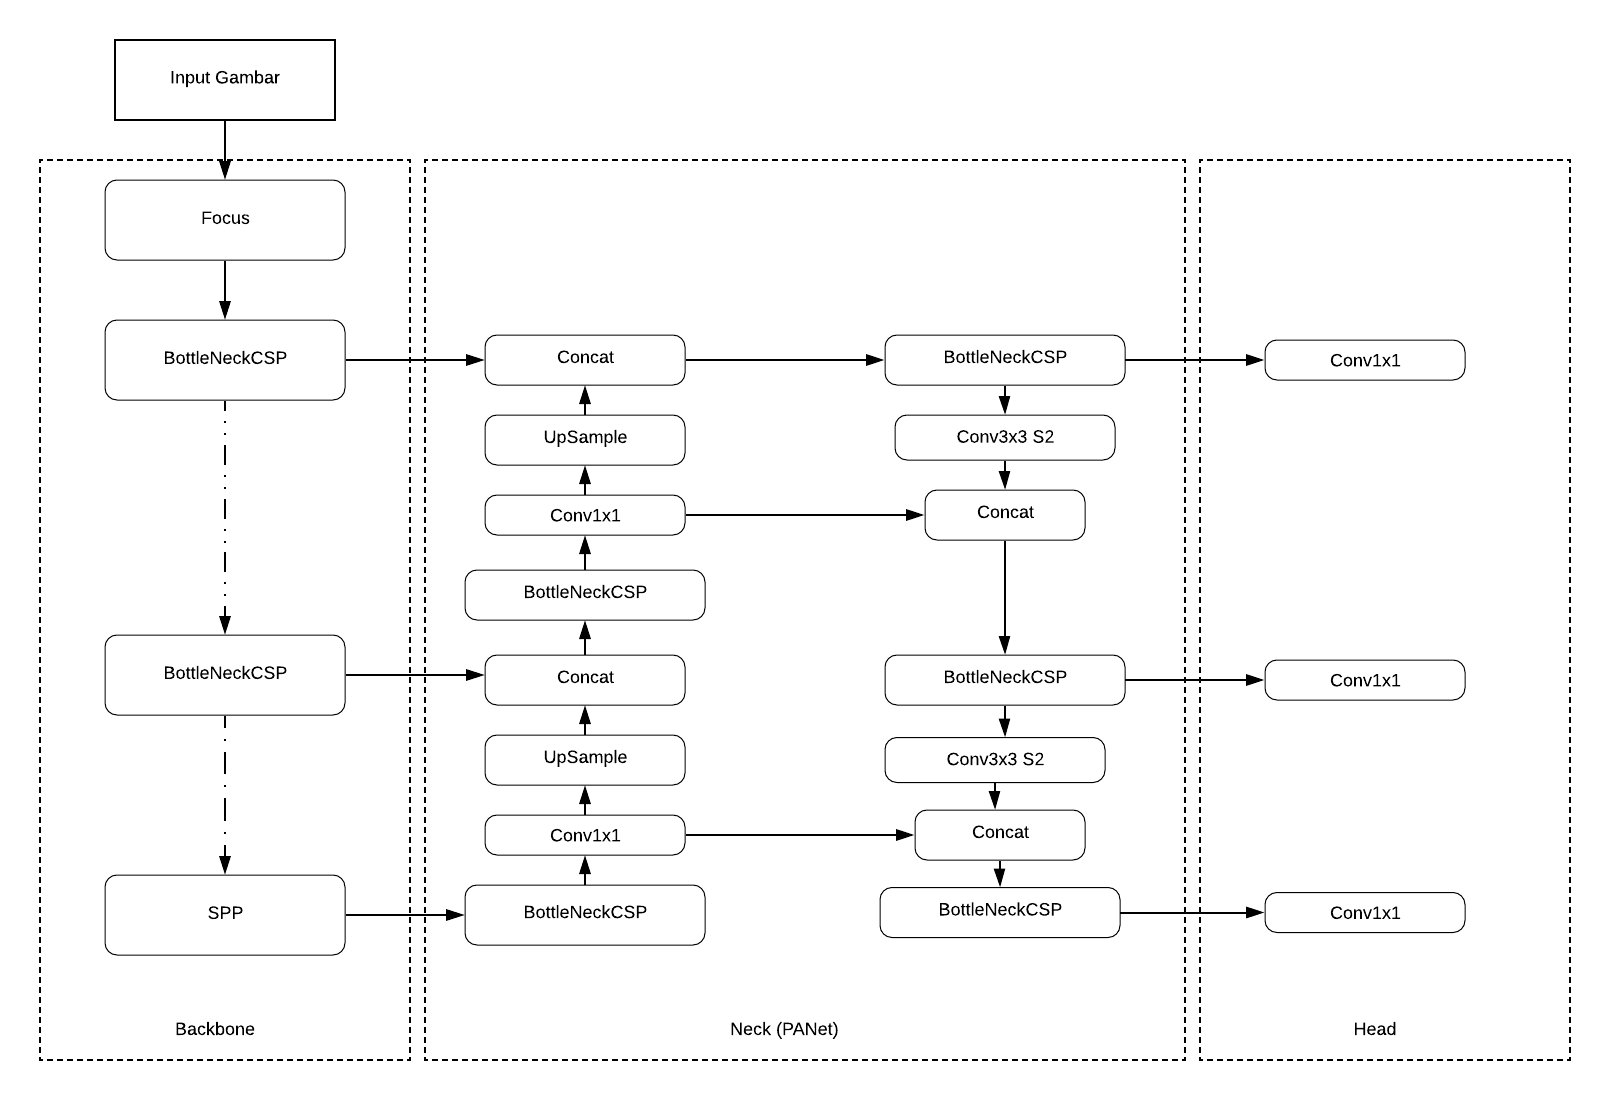
\includegraphics[width=0.9\textwidth]{gambar/yolov5 structure.png}

  % Ubah sesuai dengan keterangan gambar yang diinginkan.
  \caption{YOLOv5 Network}
  \label{fig:yolov5network}
\end{figure*}

\subsection{Tools and Equipment}
\label{subsec:toolsandequipment}

\par In working on the title of this research, there are several tools and equipments used in order to complete this research, ranging from tools in the form of software and hardware. The following is a description of the tools used.

\begin{enumerate}[nolistsep]
  \item Desktop Computer
  \item Google Colab
  \item Jetson Nano
  \item Webcam Nemesis NYK A-90 Everest
\end{enumerate}

\begin{table} [ht]
  \caption{Desktop Computer Specification}
  \label{tab:desktopspec}
  \centering
  \begin{tabular}{|c|c|}
    \hline
    % \rowcolor[HTML]{C0C0C0}
    \textbf{Type} & \textbf{Detail}  \\
    \hline
    \textit{Processor} & AMD Ryzen 5 2600 \\ 
    Memory             & 16 GB  \\
    Storage            & HDD 1TB SSD 1,256 TB\\
    Graphic Card       & NVIDIA GeForce GTX 1060 6GB \\
    Operating System   & Windows 10     \\
    CUDA               & CUDA version 11.2    \\              
    \hline
  \end{tabular}
\end{table}

\begin{table} [ht]
  \caption{Jetson Nano Specification}
  \label{tab:jetsonspec}
  \centering
  \begin{tabular}{|c|c|}
    \hline
    \textbf{Type} & \textbf{Detail}  \\
    \hline
    \textit{Processor} & Quad-core ARM Cortex-A57 MPCore processor \\ 
    Memory             & 4 GB 64-bit LPDDR4, 1600MHz 25.6 GB/s  \\
    Storage            & SDCARD 512 GB\\
    Graphic Card       & NVIDIA Maxwell architecture \\
                      & with 128 NVIDIA CUDA® cores \\
    Operating System   & Ubuntu     \\
    CUDA               & CUDA version 10.2.300    \\              
    \hline
  \end{tabular}
\end{table}

\begin{table} [ht]
  \caption{Nemesis NYK A-90 Everest Webcam Specification}
  \label{tab:nyka90_webcam_spec}
  \centering
  \begin{tabular}{|c|c|}
    \hline
    % \rowcolor[HTML]{C0C0C0}
    \textbf{Type} & \textbf{Detail}  \\
    \hline
    Resolution         & 1920x1080 \\ 
    Max FPS            & 30 FPS  \\
    Other Detail       & Full 360 Degree Rotation \\
                        & Auto Focus \\
                        & Auto Exposure White Balance    \\
                      & Full HD Glass Lens    \\              
    \hline
  \end{tabular}
\end{table}

\subsection{Workflow}
\label{subsec:workflow}

\par The working procedure of the title of this final project is divided into several stages based on the methodology that has been prepared as shown in Figure~\ref{fig:hedec_method}, namely: 

\begin{enumerate}[nolistsep]  
  \item Dataset Acquisition
  \item Dataset Labeling 
  \item Dataset Preprocessing  
  \item Dataset Training with Yolov5  
  \item Hardhat Detection System Development
  \item Hardhat Detection System  Implementation 
  \item Evaluation of implementation results 
\end{enumerate}

\begin{figure*} [ht]
  \centering
  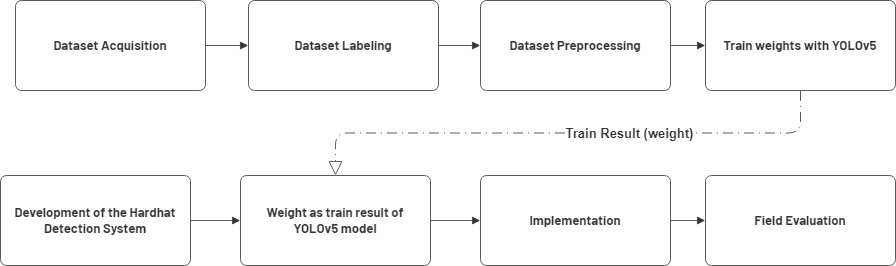
\includegraphics[width=0.9\textwidth]{gambar/utilities/methodologi_hardhat.png}

  \caption{Hardhat Detection using CNN Methodology}
  \label{fig:hedec_method}
\end{figure*}

\subsection{Dataset Acquisition}
\label{subsec:DatasetAcquisition}

\par The dataset used for training using Yolov5 is in the form of a dataset containing images containing field personnel who are wearing helmets and those who are not wearing helmets. For this study, the dataset used came from two sources, namely:

\begin{enumerate}
  \item Safety Helmet Detection by andrewmvd
  \par This dataset contains 5000 images of construction workers which including people who wear helmets and those who do not.  Each image has been labeled "helmet" and "head". The label annotation format is in the PASCAL VOC format which is stored in a .xml file. Sample of the this dataset are shown in Figure~\ref{fig:datasethelmetdetectionpreview}

  \begin{figure}[ht]
    \centering
    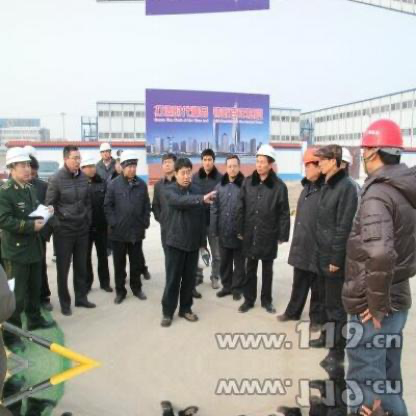
\includegraphics[width=0.24\textwidth]{gambar/sample_kaggle1/hard_hat_workers0.png}
    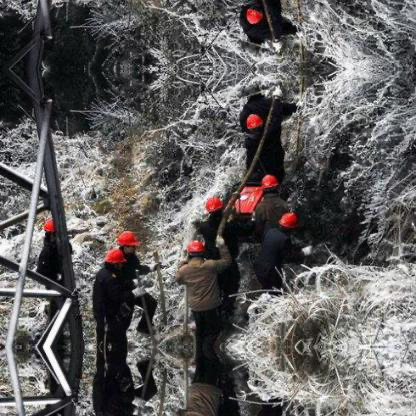
\includegraphics[width=0.24\textwidth]{gambar/sample_kaggle1/hard_hat_workers1.png}
    \caption{Dataset \emph{Safety Helmet Detection} by andrewmvd}
    \label{fig:datasethelmetdetectionpreview}  
  \end{figure}

  \item SampleERASTY2020 dataset by Alif Aditya Wicaksono
  \par This dataset contains 8,867 images whose content is similar to the previous Safety Helmet Detection dataset by andrewmvd. This dataset is also complete with annotations but requires some changes to suit the training method. In addition, the 8,867 images also include augmentation results such as flip, rotation, blur, and noise. Sample of the this dataset are shown in Figure~\ref{fig:dataseterastypreview}

  \begin{figure}[ht]
    \centering
    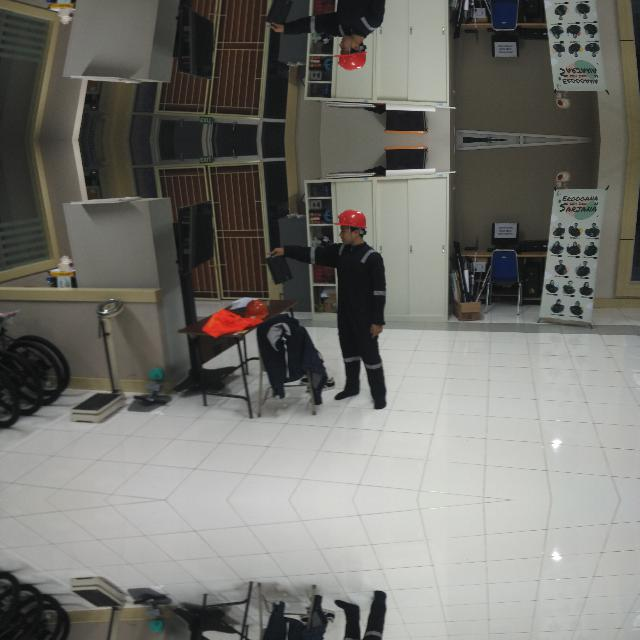
\includegraphics[width=0.24\textwidth]{gambar/sample_erasty/APB-Hat-6-_jpg.rf.79aa17f23c1834efa681edc7aca5cd5f.jpg}
    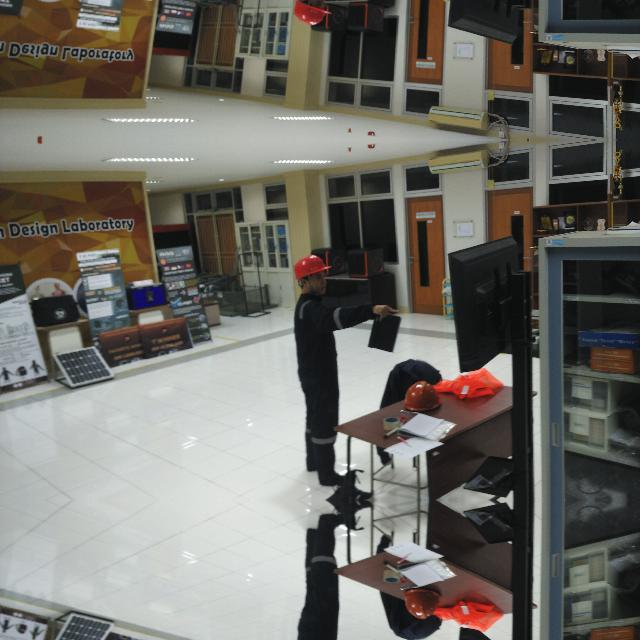
\includegraphics[width=0.24\textwidth]{gambar/sample_erasty/APB-Hat-7-_jpg.rf.4e9ff94579f598546de38a9b5c88a05d.jpg}
    \caption{Dataset SampleERASTY2020 by Alif Aditya Wicaksono}
    \label{fig:dataseterastypreview}  
  \end{figure}

\end{enumerate}

\subsection{Dataset Labeling}
\label{subsec:dataset_labeling}

\par The datasets that have been collected previously in Subsection~\ref{subsec:DatasetAcquisition} need to have annotations before being used as a training dataset. There are two classes used for this system :

\begin{enumerate}[nolistsep]
  \item "with\_helmet" which includes the head and the hardhat
  \item “no\_helmet” which includes the head without the hardhat
\end{enumerate}

\par The dataset that has been obtained already has its own labeling or annotation, but specifically for the SampleERASTY2020 dataset, there is an incompatibility for the Hard-hat label which only includes work safety helmets without the wearer's head. Therefore, a re-labeling of the SampleERASTY2020 dataset was carried out, which only used an image file that had not yet been augmented, totaling 338 images. The image labeling process is carried out on the Roboflow platform as shown in Figure~\ref{fig:gambarbesertalabel}.

\begin{figure}[ht]
  \centering
  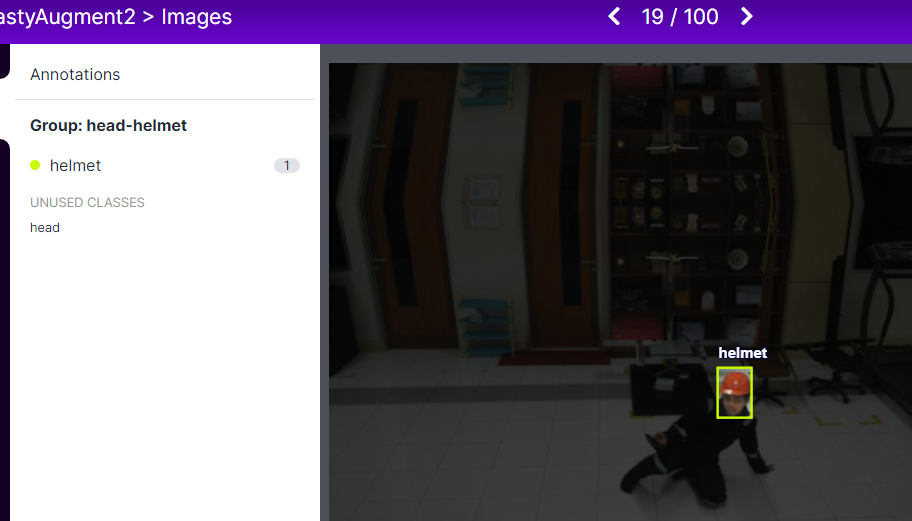
\includegraphics[width=0.4\textwidth]{gambar/utilities/labeldiroboflow.png}
  \caption{Image Labeling in Roboflow}
  \label{fig:gambarbesertalabel}  
\end{figure}

\subsection{Dataset Preprocessing}
\label{subsec:dataset_preprocessing}

\par Several processes are carried out for the datasets that have been collected so that they can be used for the training process properly. The process includes image resizing or resizing, renaming class names, and augmentation. For this research, these processes are carried out on the Roboflow platform.

\subsubsection{Image Resizing}
\label{subsec:imageresize}
\par YOLOv5 which is used to train the dataset accepts images in size 640x640 with RGB colors so the existing dataset will be resized to that size. The YOLOv5 source code from the GitHub repository already provides a resize feature before being trained but in order to preserve the image quality, the resizing process are being carried out using the Roboflow platform. 

\subsubsection{Dataset Cleanup}
\label{subsec:datasetcleanup}
\par Some images are not needed from the dataset obtained such as images that only have a safety vest which is not used for training purposes. Some of these images will not be included in the export dataset from roboflow.

\subsubsection{Class Rename}
\label{subsec:classrename}
\par The existing label class naming of the existing dataset will be adapted for easier use and understanding. The sampleERASTY2020 dataset that has been re-labeled does not need to go through this process, but the Safety Helmet Detection dataset needs to be renamed where for the “helmet” class it becomes “with\_helmet” and “head” becomes “no\_helmet” as shown in Figure \ref{fig:prepro_classrename}.

\begin{figure}[ht]
  \centering
  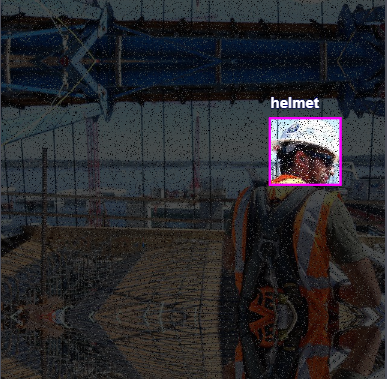
\includegraphics[width=0.24\textwidth]{gambar/utilities/reclass_old.png}
  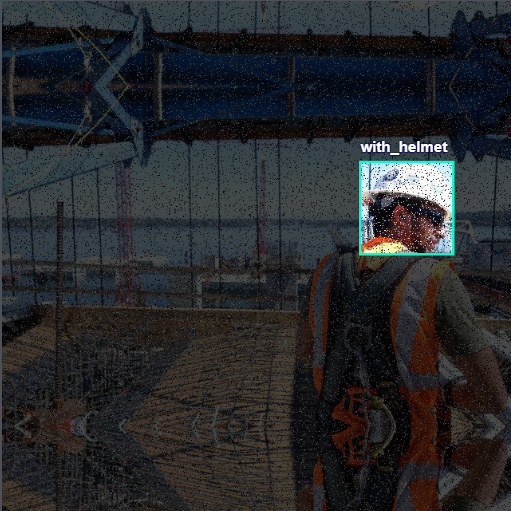
\includegraphics[width=0.24\textwidth]{gambar/utilities/reclass_new.png}
  \caption{Class Rename in Roboflow}
  \label{fig:prepro_classrename}  
\end{figure}

\subsubsection{Augmentation}
\label{subsec:augmentation}
\par Additional augmentation is also carried out on the dataset to add variations to the image in the dataset where the augmentation forms used are noise and horizontal flip as shown in Figure~\ref{fig:prepro_augmentasi}. The augmentation process is carried out on the Roboflow platform which also provides augmentation features. The re-labeled and additional augmented SampleERASTY2020 dataset was then combined with the previously obtained dataset of 5000 images of the Safety Helmet Dataset by andrewvmd.

\begin{figure}[ht]
  \centering
  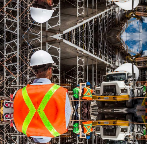
\includegraphics[width=0.24\textwidth]{gambar/utilities/aug_flip.png}
  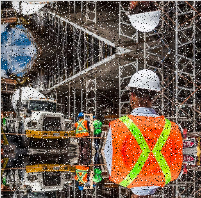
\includegraphics[width=0.24\textwidth]{gambar/utilities/aug_noise.png}
  \caption{\emph{Flip} and \emph{Noise} Augmentation}
  \label{fig:prepro_augmentasi}  
\end{figure}

\subsubsection{Dataset Subset}
\label{subsec:datasetsubset}
\par Before being used for weight training, the previously combined dataset needs to be divided into the train - test - val set. The division for the dataset used for training is 70\% train (4202) , 20\% test (1,200 images), and 10\% validation (600 images). For training using PyTorch-based YOLOv5, Roboflow provides an export dataset feature to a specified format where here the annotations are saved in the form of '.txt' and managed via a '.yaml' file. The distribution of this dataset is done through the Generate Dataset Version feature on the Roboflow platform. The dataset was obtained from the dataset merging process mentioned in Subsection~\ref{subsec:DatasetAcquisition} and after going through pre-processing.

\subsection{Training}
\label{subsec:dataset_training}

\par Datasets that have been pre-processed previously in roboflow and already have appropriate annotations are then used for training using YOLOv5. This training is a model training process with input images from annotated datasets where the images and annotations are processed to produce a special characteristic or pattern from a predetermined class/label through annotations so that the computer can then use the computer to guess the image that will be detected. . Especially for YOLOv5 which uses PyTorch as its machine learning framework, the training results in the form of weights will be exported in the form of '.pt' (pytorch format).

\begin{table} [ht]
  \caption{Train Configuration}
  \label{tb:trainconfig}
  \centering
  \begin{tabular}{|c|c|}
    \hline
    % \rowcolor[HTML]{C0C0C0}
    \textbf{Parameters} & \textbf{Detail}  \\
    \hline
    \emph{batch\textunderscore size} & 16 \\
    \emph{epoch} & 150 \\
    \emph{imgsize} & 640\\
    % \emph{data} & /content/yolov5/helmetDetection\textunderscore yolov5\textunderscore 2/data.yaml\\
    \emph{optimizer} & SGD (DEFAULT)\\
    \emph{device} & CUDA\\  
    \hline
  \end{tabular}
\end{table}

\par As can be seen in Table~\ref{tb:trainconfig}, the training process is carried out with batch sizes of 16 and 150 epochs with the default optimizer for yolov5 which is SGD. Batch\textunderscore size here determines the number of images that will be used to train in one iteration, determined 16 by considering the hardware limitations used for this training process. The training process is carried out in Colab Pro were with the given GPU Ram limitation, it is used up to 12 GB. For the image size itself, the algorithm provided by YOLOv5 only provides a 1:1 resolution whereby specifying the imgsize parameter 640 means the size for (height) and (width) becomes 640x640.

\par The training process in this research is carried out by utilizing pretrained weights provided from the YOLOv5 repository and also without using these pretrained weights with the aim of comparing the performance of the weights generated from these methods but will use a configuration similar to the configuration used to -train the pretrained weights. The weight variants that will be used are yolov5n (Nano), yolov5s (Small), yolov5m (Medium), and yolov5l (Large) variants. Based on the explanation from the YOLOv5 repository, the pretrained weights provided are the result of training using the COCO val2017 dataset parameter 300 epoch \cite{glenn_jocher_yolov5}. The main difference between these pretrained weights is in the "depth\_multiplier" and "width\_multiplier" parameters which have an impact on the layer depth and the number of channels of output for each layer. The nominal configuration of "depth\_multiplier" and "width\_multiplier" for each variant can be seen in the table.

\begin{table} [ht]
  \caption{depth\_multiplier and width\_muliplier Difference}
  \label{tb:pretrainedparamdiff}
  \centering
  \begin{tabular}{|l|l|l|}
    \hline
    \multirow{2}{*}{Model Name} & \multicolumn{2}{l|}{Multiplier}      \\ 
    \cline{2-3}
                                 & depth\_multiplier & width\_muliplier  \\ 
    \hline
    yolov5n\textit{ (Nano)}      & 0.33              & 0.25              \\
    yolov5s\textit{ (Small)}     & 0.33              & 0.5               \\
    yolov5m\textit{ (Medium)}    & 0.67              & 0.75              \\
    yolov5l\textit{ (Large)}     & 1                 & 1                 \\
    \hline
  \end{tabular}
\end{table}

\par The training process for this title is not carried out with local computer hardware but uses Google Colab Pro where the training process is run in the cloud. The previously collected dataset is downloaded to the Colab Pro vm storage directly from Roboflow. With limitations on the use of storage, ram, and GPU ram as well as runtime provided by Google Colab, checkpoints are stored for each training epoch on the author's drive. This is done for the possibility that in the middle of the VM Colab Pro training session, the VM Colab Pro terminates automatically on itself. 

\subsection{Development of The Hardhat Detection System}
\label{subsec:hedect_dev_sys}

\par This hardhat detection system will utilize YOLOv5 to make predictions on the input received. Input is an image received from a webcam or camera connected to a computer that will run this system. The system was developed with the aim of detecting the use of work safety helmets in real-time and will run an alarm mechanism if on the camera input there is someone who is not wearing a work safety helmet. The flowchart for the Safety Helmet Detection system can be seen at Figure~\ref{fig:flowchart_sistem}.

\par The system will be created as a python script file that can be run and can accept several parameters: input source, weight to be used, confidence threshold, and IoU threshold for the Non Max Suppression process.

\par Input that can be used with the created script can be done in the form of video files or camera feeds. The system can accept various resolutions, but for the inference process, the input dimensions will be resized to 640x640 and the output will be adjusted to the dimensions of the initial input.

\par Each frame that comes in from the input webcam will be used to process inference via
yolov5 model with weight that has been created previously through the training process.
The result of inference using YOLOv5 will return the input in the form of position for
the detected object is in xcenter, ycenter and the dimension of the object is in widht
and height as well as the name information class and confidence score for
each detected object. The result of output inference obtained is then used to draw
bounding box on the frame image being inference
as in Figure~\ref{fig:bboxresult}.

% Contoh input gambar pada kolom.
\begin{figure} [ht]
  \centering
  % Ubah sesuai dengan nama file gambar dan ukuran yang akan digunakan.
  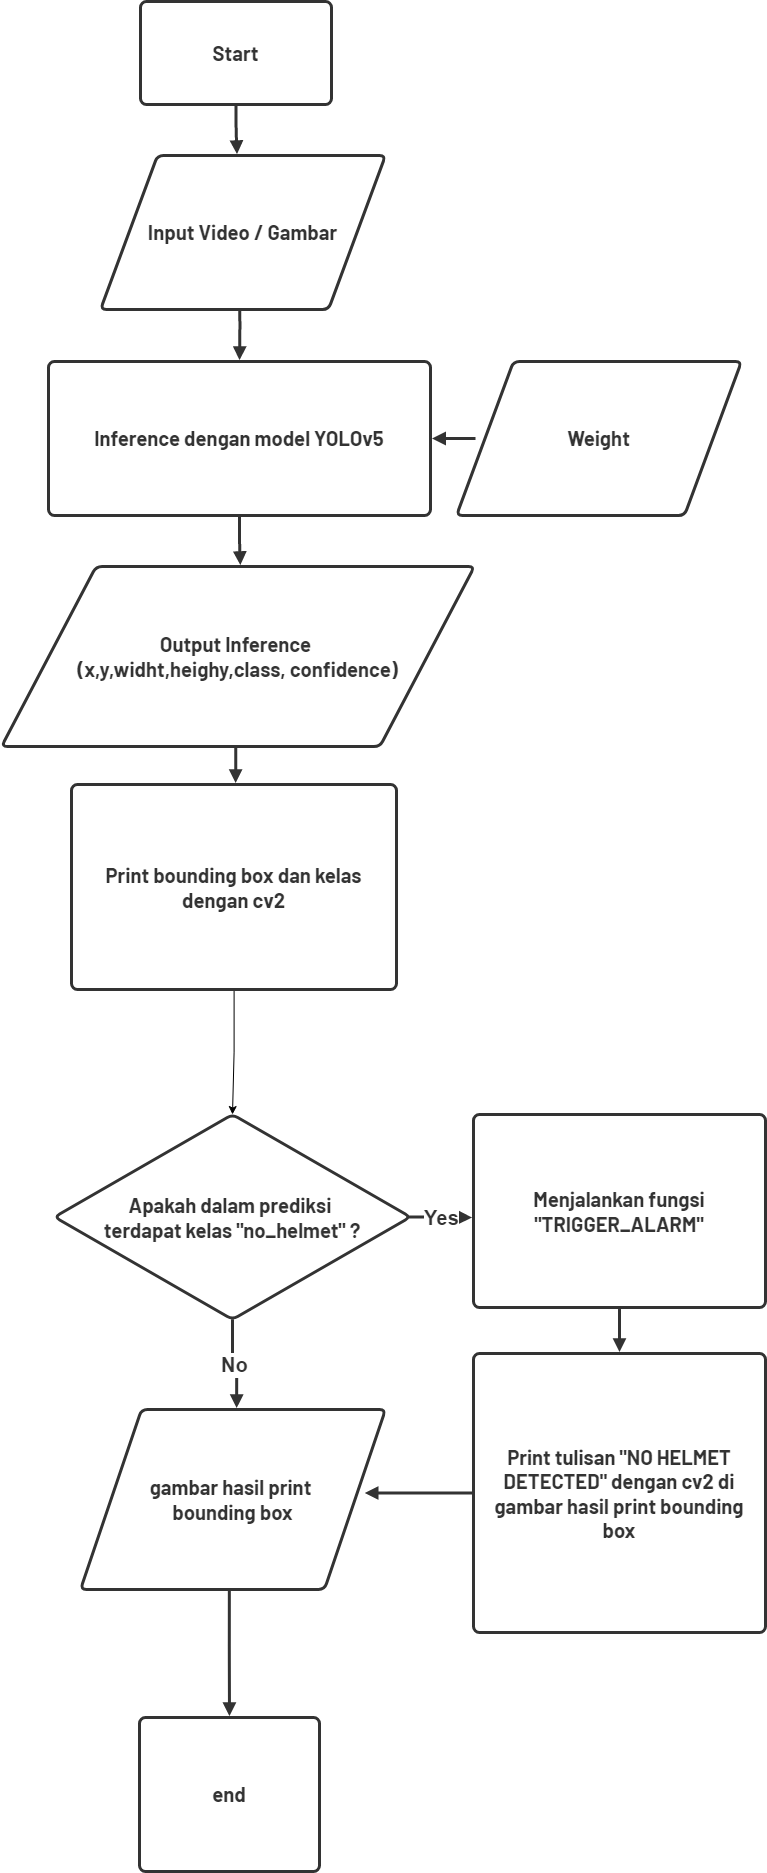
\includegraphics[width=0.4\textwidth]{gambar/utilities/sistemhedect.drawio.png}

  % Ubah sesuai dengan keterangan gambar yang diinginkan.
  \caption{Hardhat Detection System Flowchart}
  \label{fig:flowchart_sistem}
\end{figure}

\begin{figure} [ht]
  \centering
  % Ubah sesuai dengan nama file gambar dan ukuran yang akan digunakan.
  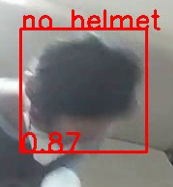
\includegraphics[width=0.2\textwidth]{gambar/utilities/bbox1.png}
  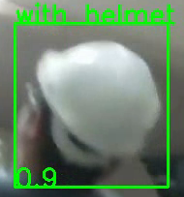
\includegraphics[width=0.2\textwidth]{gambar/utilities/bbox2.png}

  % Ubah sesuai dengan keterangan gambar yang diinginkan.
  \caption{Bounding Box Result}
  \label{fig:bboxresult}
\end{figure}


\par The alarm function will be executed when one or more 'no\_helmet' 
class object is detected inside the frame that is being \emph{inferenced} by the model. 
This alarm function contains commands to play the alarm audio to simulate a siren alarm. 
In addition to running the alarm function, it will also run a command to display 
“NO\_HELMET DETECTED” on the predicted frame as shown in Figure~\ref{fig:alarmtriggerexample}.

\begin{figure} [ht]
  \centering
  % Ubah sesuai dengan nama file gambar dan ukuran yang akan digunakan.
  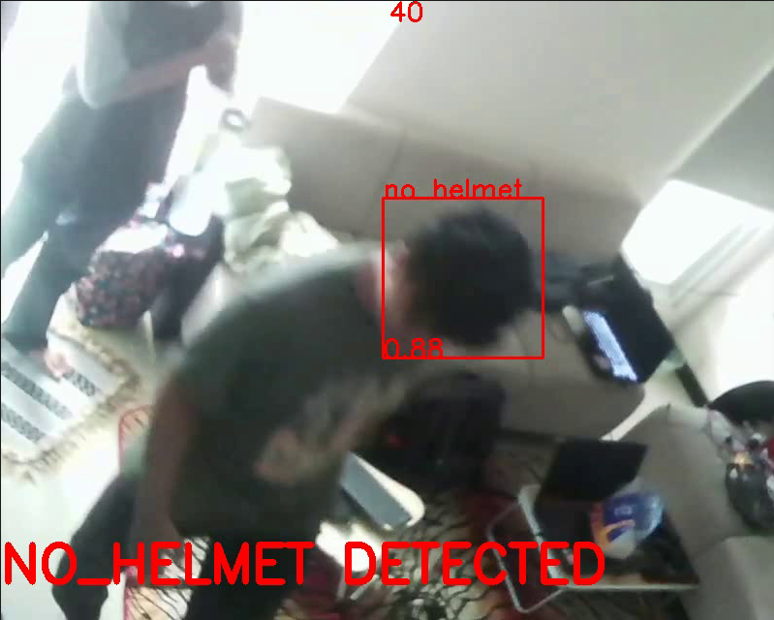
\includegraphics[width=0.4\textwidth]{gambar/utilities/alarm_example.png}

  % Ubah sesuai dengan keterangan gambar yang diinginkan.
  \caption{Example On Alarm Trigger}
  \label{fig:alarmtriggerexample}
\end{figure}

\par As an addition, the Frame-rate counter will be shown on the middle top of the window 
of the output. This is done as a way to benchmark the performance of each model that 
is being tested in this research where YOLOv5 provides a Small variant to a Large variant. 
It is expected the larger the model, the smaller the frame per second (FPS) will be.